\noindent Recall that some diagrams evaluate to infinity in the calculation of the time-ordered $n$-point correlation function
\begin{equation}
G^{(n)}(\textbf{x}_1,\dots,\textbf{x
}_n) = \bra{\Omega} \mathcal{T}[\hat{\phi}(\textbf{x}_1) \dots \hat{\phi}(\textbf{x}_n) ] \ket{\Omega} = \left( {\tiny \stackanchor{sum over all connected diagrams}{with $n$ external points/legs} } \right)
\end{equation}

\subsection*{Example: $n=4$ Diagrams}

\noindent For example, the $n=4$ case sums over diagrams like the following

\begin{figure}[H]
	\centering
	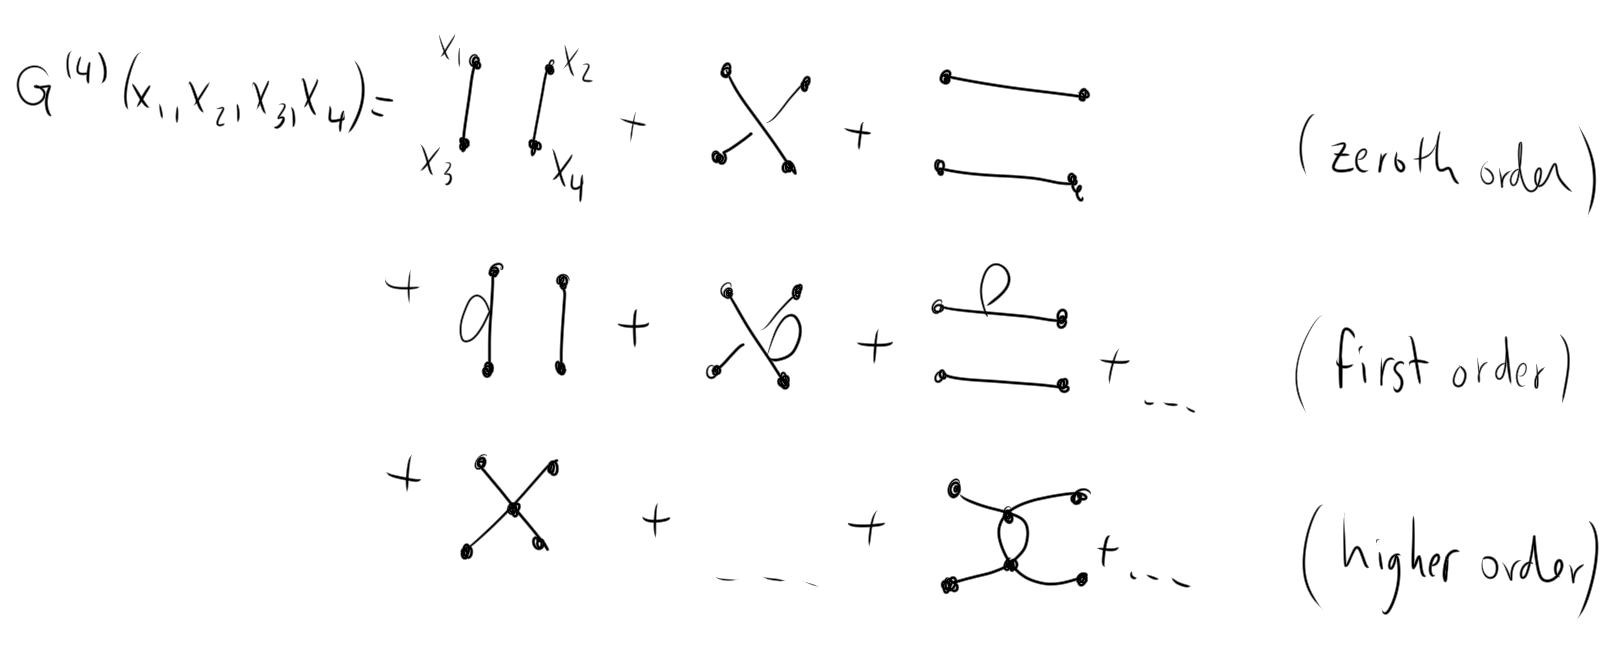
\includegraphics[scale=0.4]{g4.png}
	\caption{Sum over connected diagrams for $n=4$ case.}
\end{figure}

\noindent Diagrams with one loop (\textit{first order}) evaluate to infinity, but are easily eschewed. Two vertex diagrams (last one in figure above) is a much more difficult infinity to tame, and causes divergences, typically of the form, in momentum space,
\begin{equation}
\mathcal{I} = \int \frac{d^4 p} {(2\pi)^4} \, \frac{i}{\textbf{p}^2-m^2+i\epsilon}
\end{equation}

\noindent To attempt to tame the infinity, impose a cutoff at scale $\Lambda$
\begin{equation}
\mathcal{I} \to \mathcal{I}(\Lambda) = \int_{|p| < \Lambda} \frac{d^4 p} {(2\pi)^4} \, \frac{i}{\textbf{p}^2-m^2+i\epsilon} .
\end{equation}

\noindent To cope with arbitrary choices of $\Lambda$, arbitrary coupling constants can be employed to compensate and remove possible $\Lambda$-dependencies in calculations. Further explanation can be found in the renormalization theory of scalar particles.

\subsection*{Scattering Theory}

\noindent Scattering theory is an effective theory for large time limits $|t| >> \text{constant}$. The probability of a scattering event occuring, the scattering amplitude, in the case of well-collimated beams with incoming momenta $\textbf{k}_A$ and $\textbf{k}_B$, and outgoing momenta $\textbf{p}_j, \, j=1,\dots,n$, is related to the quantity
\begin{equation}
_{out}\braket{\textbf{p}_1 \textbf{p}_2 \dots \textbf{p}_n | \textbf{k}_A \textbf{k}_B}_{in} = \bra{\textbf{p}_1 \textbf{p}_2 \dots \textbf{p}_n} \mathcal{S} \ket{\textbf{k}_A \textbf{k}_B} .
\end{equation}

\begin{figure}[H]
	\centering
	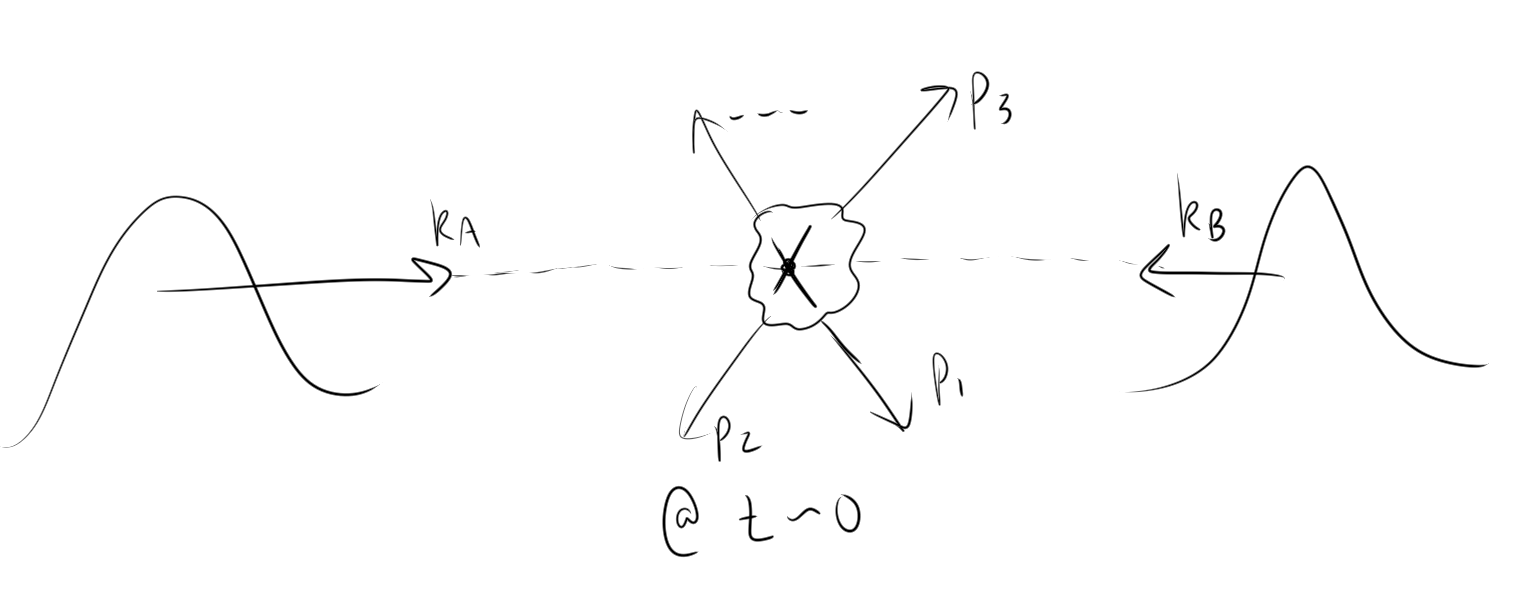
\includegraphics[scale=0.4]{scattering.png}
	\caption{Schematic of scattering experiment with incoming momenta and outgoing momenta as described above.}
\end{figure}

\noindent For the free, non-interacting, theory, we have the equation for incoming momenta related to the free vacuum state, denoted by $\ket{\,}_0$,
\begin{equation}
\ket{k_A k_B}_{in} = \sqrt{2 \omega_{k_A} \omega_{k_B}} \hat{a}_{k_A}^\dagger \hat{a}_{k_B}^\dagger \ket{0}_0 .
\end{equation}

\noindent The task at hand is to calculate the scattering amplitude $\bra{\textbf{p}_1 \textbf{p}_2 \dots \textbf{p}_n} \mathcal{S} \ket{\textbf{k}_A \textbf{k}_B}$. Define the $\mathcal{S}$-matrix as
\begin{equation}
\mathcal{S} = \mathbb{I} + i \hat{\mathbb{T}}.
\end{equation}

\noindent Where the identity $\mathbb{I}$ is the dominant term in small intercation, where almost nothing happens, and the operator $\hat{\mathcal{T}}$ is the dominant in larger interactions. Introduce the quantity $\mathcal{M}$ to factor out the conservation of momentum in the scattering process, where all momenta are "on shell", such that $\textbf{p}^0 = \omega_p$. 
\begin{equation}
\bra{\textbf{p}_1 \dots \textbf{p}_n} i\hat{\mathbb{T}} \ket{\textbf{k}_A \textbf{k}_B} = (2\pi)^4 \delta^{(4)}((\textbf{k}_A + \textbf{k}_B) - \sum_{j=1}^{n} p_j) \cdot i \mathcal{M}((\textbf{k}_A, \textbf{k}_B) \to \textbf{p}_f).
\end{equation}

\noindent Recall that the differential scattering cross section of $2\to 2$ particles in the center of mass frame is
\begin{equation}
\left( \frac{d\sigma}{d\Omega}\right)_{CM} = \frac{|\mathcal{M}|^2}{64 \pi^2 E^2_{CM}}
\end{equation}

\noindent To compute the scattering amplitude $\bra{\textbf{p}_1 \textbf{p}_2 \dots \textbf{p}_n} \mathcal{S} \ket{\textbf{k}_A \textbf{k}_B}$, take "on faith" that for small interactions
\begin{equation}
\ket{k_A k_B}_{int} \propto \lim_{t\to\infty} e^{-i\hat{H}t} \ket{k_A k_B}_0 .
\end{equation}

\noindent And compare this to the result related to the Riemann-Lebesgue lemma
\begin{equation}
\ket{\Omega}_{int} = \lim_{t\to\infty} e^{-i\hat{H}t} \ket{0}_0 . 
\end{equation}

\noindent An argument for the plausibility for the second equality of $\ket{\Omega}_{int}$, where $\hat{H} = \hat{H}_{KG} + \hat{H}_{int}$, $\hat{H}_{KG}\ket{0}_0 = 0$, and $\hat{H}\ket{\Omega}_{int} = 0$, is as follows. Suppose that the Hamiltonian is parameterized by $s \in [0,1]$, such that $\hat{H}(s) = \hat{H}_{KG} + s \hat{H}_{int}$, and that the free Hamiltonian $\hat{H}_{KG}$ has a spectral gap of $\Delta(s)=m$. When $s=0$, we have the free, Klein-Gordon Hamiltonian, and when $s=1$, we have the interacting, $\varphi^4$ Hamiltonian. Then it's plausible that the spectral gap in the spectrum of eigenvalues of $\hat{H}(s)$ will always be nonzero for at least just one eigenvalue, and the spectrum is adiabatically connected (can't instantaneously go from massful to massless, but interactions can be turned on/off gradually). \\

\begin{figure}[H]
	\centering
	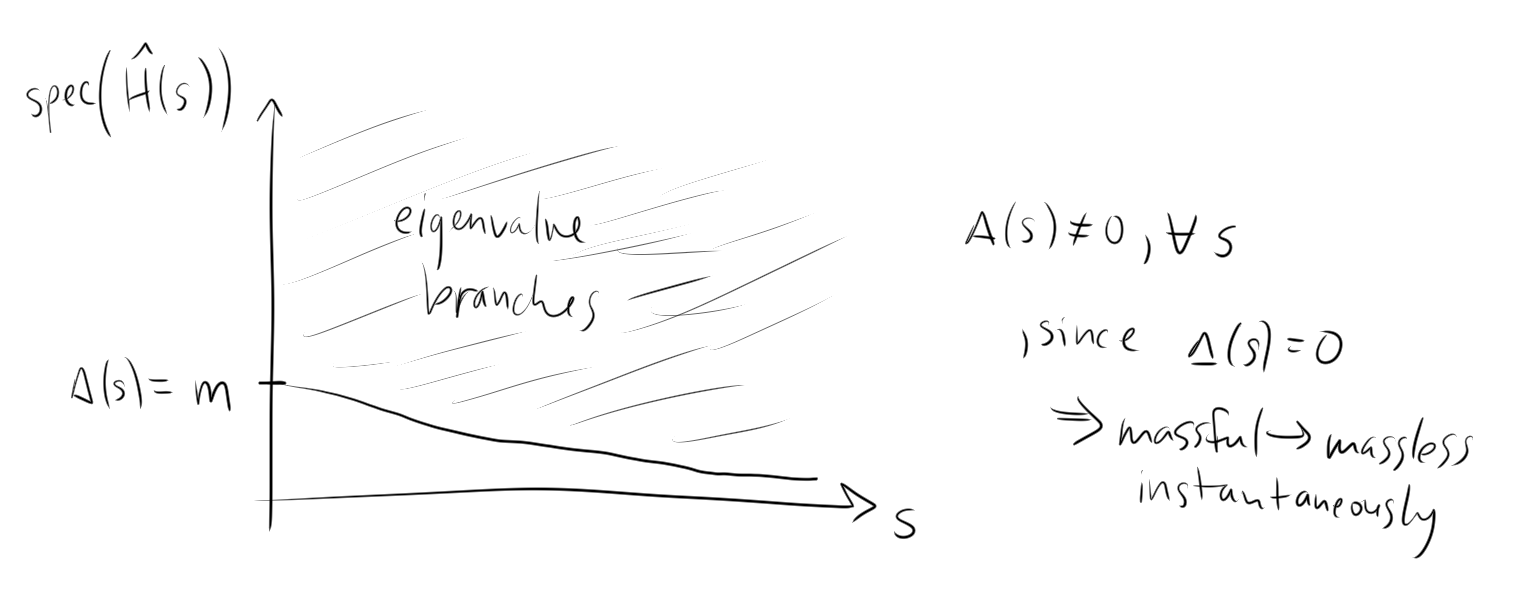
\includegraphics[scale=0.4]{eivs.png}
	\caption{Schematic of the spectral gap for the parameterized Hamiltonian.}
\end{figure}

\noindent For the proportionality factor of $\ket{k_A k_B}_{int}$ to be true for small interactions, which is far more radical, it is required that there are nonzero spectral gaps, for some $s>0$, at each momentum eigenstate of momenta $\textbf{k}_A$ and $\textbf{k}_B$, and there are no other nearby eigenvalues that may be mistaken for the incoming momenta. In practice, these incoming particles can create bound states, for example, and make this distinction difficult. If all of this is justifiable, and we accept the proportionality $\ket{k_A k_B}_{int} \propto \lim_{t\to\infty} e^{-i\hat{H}t} \ket{k_A k_B}_0$, then we can create equalities and proportionalities, although difficult, to quantities that we can actually calculate
\begin{equation}
\lim_{t\to\infty} \,_{0}\bra{\textbf{p}_1 \dots \textbf{p}_n} e^{-i hat{H} \cdot 2t} \ket{\textbf{k}_A \textbf{k}_B}_0 \propto \lim_{t\to\infty} \,_{0}\bra{\textbf{p}_1 \dots \textbf{p}_n} \mathcal{T}[ e^{-i \int^t_{-t} \hat{H}_{int}(t')dt'}] \ket{\textbf{k}_A \textbf{k}_B}_0
\end{equation}

\noindent This is exactly the same as the argument for the Dyson series expansion for $G^{(n)}$ with the vacuum states, and, just as in that case, the proportionality difficulty can be eliminated, and we have the following (not yet justified) equality
\begin{equation}
\bra{\textbf{p}_1 \dots \textbf{p}_n} i\hat{\mathbb{T}} \ket{\textbf{k}_A \textbf{k}_B} = \lim_{t\to\infty} \left( \,_{0}\bra{\textbf{p}_1 \dots \textbf{p}_n} \mathcal{T}[ e^{-i \int^t_{-t} \hat{H}_{int}(t')dt'}] \ket{\textbf{k}_A \textbf{k}_B}_0 \right)_{\tiny \stackanchor{connected,}{amputated}}
\end{equation}

\noindent The condition of "connected, amputated" is analogous to "connected" as in the $G^{(n)}$ case. \\

\noindent We can begin to justify this equality through some calculations. Consider the $\mathcal{O}(1)$ term, corresponding to the identity operator in  $\mathcal{S} = \mathbb{I} + i \hat{\mathbb{T}}$, for the $2\to 2$ scattering process.
\begin{align}
_{out}\braket{\textbf{p}_1 \textbf{p}_2 | \textbf{k}_A \textbf{k}_B}_{in} &=_{\mathcal{O}(1)} \,_{0}\braket{\textbf{p}_1 \textbf{p}_2 | \textbf{k}_A \textbf{k}_B}_{0} \\
&= \sqrt{2\omega_{p_1}\omega_{p_2}\cdot 2 \omega_{k_A}\omega_{k_B}} \bra{0} \hat{a}_{p_1} \hat{a}_{p_2} \hat{a}_{k_A}^\dagger \hat{a}_{k_B}^\dagger \ket{0} \\
&= 2\omega_A \cdot 2\omega_B (2\pi)^6 (\delta(\textbf{p}_1-\textbf{k}_A)\delta(\textbf{p}_2-\textbf{k}_B) + \delta(\textbf{p}_1-\textbf{k}_B)\delta(\textbf{p}_2-\textbf{k}_A))
\end{align}

\begin{figure}[H]
	\centering
	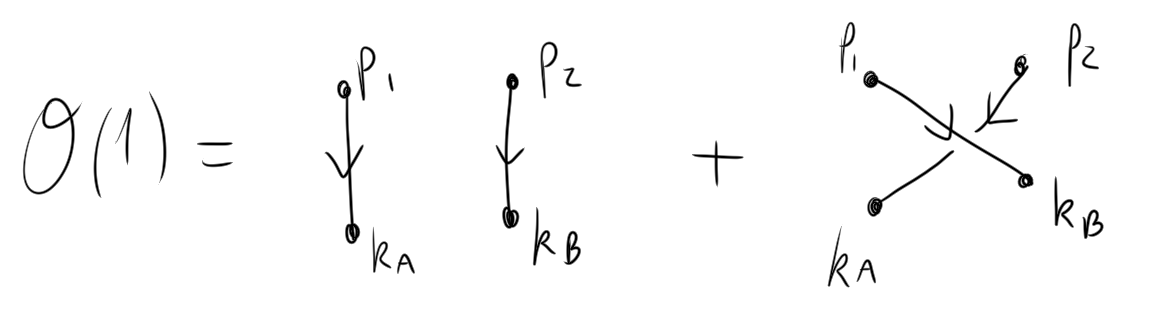
\includegraphics[scale=0.4]{o1.png}
	\caption{Diagram of the $\mathcal{O}(1)$ term as calculated above.}
\end{figure}

\noindent The next term to $\mathcal{O}(\lambda)$, applying Wick's theorem, and retaining all contractions, since we are not just working with the vacuum state anymore,
\begin{align}
\bra{\textbf{p}_1 \textbf{p}_2} i\hat{\mathbb{T}} \ket{\textbf{k}_A \textbf{k}_B}  &=_{\mathcal{O}(\lambda)} \,_{0}\bra{\textbf{p}_1 \textbf{p}_2} \mathcal{T}[ \frac{-i\lambda}{4!} \int d^4 x \, \hat{\phi}_I^4(\textbf{x}) ] \ket{\textbf{k}_A \textbf{k}_B}_{0} \\
&= \,_{0}\bra{\textbf{p}_1 \textbf{p}_2} \mathcal{N}[ \frac{-i\lambda}{4!} \int d^4 x \, \hat{\phi}_I^4(\textbf{x}) + {\tiny \stackanchor{all}{contractions}}\, ] \ket{\textbf{k}_A \textbf{k}_B}_{0}
\end{align}

\noindent To see what kinds of terms that survive to order $\lambda$, consider the interacting creation field operator interacting with the free four-momentum eigenstate
\begin{align}
\hat{\phi}_I^\dagger(\textbf{x}) \ket{\textbf{p}}_0 &= \int \frac{d^3 k}{(2\pi)^3} \, \frac{1}{\sqrt{2 \omega_k}} e^{-i \textbf{k}\cdot\textbf{x}} \hat{a}_k \ket{p} \\
&= \int \frac{d^3 k}{(2\pi)^3} \, \frac{1}{\sqrt{2 \omega_k}} e^{-i \textbf{k}\cdot\textbf{x}} \hat{a}_k \cdot \sqrt{2 \omega_p} \hat{a}_p^\dagger \ket{0} \\
&= \int \frac{d^3 k}{(2\pi)^3} \, \frac{1}{\sqrt{2 \omega_k}} e^{-i \textbf{k}\cdot\textbf{x}} \cdot (2\pi)^3 \delta^{(3)}(k-p) \sqrt{2\omega_p} \ket{0} \\
\hat{\phi}_I^\dagger(\textbf{x}) \ket{\textbf{p}}_0 &= e^{-i p\cdot x} \ket{0} .
\end{align}

\noindent To deal with momentum eigenstates, such as $\ket{\textbf{k}_A \textbf{k}_B}$, include them in \textit{extended contractions} by defining
\begin{align}
\wick[offset=1.5em]{\c {\hat{\phi}_I^\dagger(\textbf{x})} \c {\ket{p}} } &= e^{-i \textbf{p}\cdot \textbf{x}} \\
\wick[offset=1.5em]{\c {\bra{p}} \c {\hat{\phi}_I^\dagger(\textbf{x})}} &= e^{i \textbf{p}\cdot \textbf{x}}
\end{align}

\noindent Now, we can prove (\textbf{Exercise}) an extended version of Wick's theorem, where the time-ordered product of field operators in the presence of incoming and outgoing momentum eigenstates is equal to the sum over all possible contractions, including contractions of the field operators with the states as well.
\begin{equation}
_{0}\bra{\textbf{p}_1 \dots \textbf{p}_n} \mathcal{T}[{\small\text{field operators}}] \ket{\textbf{k}_1 \dots \textbf{k}_n} _{0} = \sum {\tiny \stackanchor{all possible full contractions}{including momentum eigenstates}}
\end{equation}

\noindent This allows us to approximate the $\mathcal{S}$-matrix transition amplitudes, justified up to the assumption about momentum eigenstates in the free theory being related to momentum eigenstates in the interacting theory.